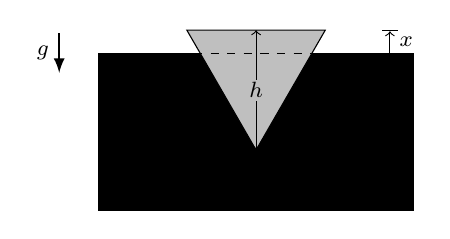
\begin{tikzpicture} [
	scale=1,
	font=\footnotesize,
	vecteur/.style={-latex,thick},
	liquide/.style={fill=\JRLblueC,very thin,draw=\JRLblueF},
    solide/.style={fill=lightgray},
	]
	% liquide
	\draw[liquide] (-2,0)--++(4,0)--++(0,-2)--++(-4,0)--cycle;
	\draw (-2,0)--++(4,0);
	\draw (0,-1.75) node{eau ($\rho_\text{e}$)};
	% solide
	\draw[solide,shift={(0,-35pt)}](0,0)--(120:50pt)--++(0:50pt)--cycle;
	\draw[dashed,thin] (-1,0)--++(2,0);
	\draw[shift={(0,-35pt)},<->](0,0)--++(0,43.3pt)node[inner sep=1pt,midway,fill=lightgray]{$h$};
	\draw[->|](1.7,0)--++(0,8.3pt)node[midway,right]{$x$};
	% forces
	\draw[vecteur] (-2.5,0.25)--++(0,-0.5) node[pos=0.5,left]{$\vv{g}$};
	% \draw[help lines] (-2,-2) grid (2,2);
\end{tikzpicture}